\documentclass{standalone}
\usepackage{mathpazo}
\usepackage{tikz}
\usetikzlibrary{calc}

\begin{document}
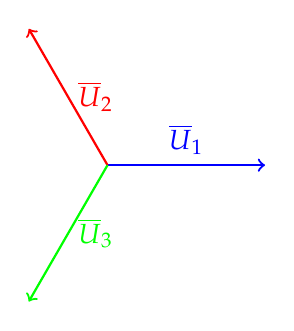
\begin{tikzpicture}
  \draw (0,0) coordinate (N);
  \draw[->, color=blue, thick] (N) -- (0:2) node[above, midway] {$\overline{U}_1$};
  \draw[->, color = red, thick] (N) -- (120:2) node[right, midway] {$\overline{U}_2$};
  \draw[->, color = green, thick] (N) -- (-120:2) node[right, midway] {$\overline{U}_3$};
\end{tikzpicture}
\end{document}